% Provenance (never printed): the price-level strand of ../economics_series.md (grade 8: basket, index, inflation rate,
% nominal and real, hyperinflation and deflation; the monetary cause of inflation belongs to the grades 10-12 volume).
% Brief: sources/book1/BRIEFS.md, g8-03. Chart data: figdata/grade-8/03-inflation-and-price-indices (JST cpi; BLS CPI-U;
% Brenland basket). Ledger: g8:rentenmark-issue, g8:rentenmark-rate, g8:rentenmark-dollar.
\chapter{Inflation and Price Indices}\label{ch:g8:inflation-and-price-indices}

\begin{openingchart}{Consumer-price inflation in four countries, each year from 1920 to 2020,
in percent. Japan's inflation of 1945--1948 goes far above the top of the chart (up to $975.6\,\%$
in 1945).}{Jord\`a--Schularick--Taylor Macrohistory Database, \omterm{def:g8:inflation-and-price-indices:cpi}{consumer price index}}
\begin{tikzpicture}
\begin{axis}[omtime, xmin=1920, xmax=2020, ymin=-20, ymax=60, restrict y to domain=-30:200,
  xtick={1920,1940,1960,1980,2000,2020}, xlabel={Year}, ylabel={Inflation (percent)},
  legend style={at={(0.5,-0.2)}, anchor=north, legend columns=4}, extra y ticks={0},
  extra y tick style={grid=major, grid style={black!60}}]
\pgfplotsforeachungrouped \col in {usa, gbr, fra, jpn} {
  \addplot+[thin] table[x=year, y=\col] {figdata/grade-8/03-inflation-and-price-indices/out/inflation_century.csv};
}
\legend{United States, United Kingdom, France, Japan}
\end{axis}
\end{tikzpicture}
\end{openingchart}

% figdata: facts (usa_1921 -10.5, usa_1932 -9.9, jpn_1945 975.6, fra_1948 58.6, gbr_1975 22.7, usa_1980 11.2,
% jpn_2009 -1.3, deflation_years_usa 13, deflation_years_jpn 24; us_inf_2021 4.7, us_inf_2022 8.0, us_inf_2025 2.6)
For a hundred years, \omterm{def:g7:money:price}{prices} in these four countries have mostly risen. In some years they rose
fast: $58.6\,\%$ in France in 1948, $22.7\,\%$ in the United Kingdom in 1975, $11.2\,\%$ in the United
States in 1980. In Japan in 1945, \omterm{def:g7:money:price}{prices} were on average almost eleven times their level of
1944. In other years \omterm{def:g7:money:price}{prices} fell: by $10.5\,\%$ in the United States in 1921, by $9.9\,\%$
in 1932. From 1993 to 2020, inflation in the four countries stayed below $5\,\%$; \omterm{def:g7:money:price}{prices} in
Japan fell in 24 of the hundred years, many of them after 1995. More recent data from the United
States show inflation of $4.7\,\%$ in 2021, $8.0\,\%$ in 2022, and $2.6\,\%$ in 2025.

How can one number say how much ``\omterm{def:g7:money:price}{prices}'' rose, when the \omterm{def:g7:money:price}{price} of bread, rent and fuel each
change differently? This chapter builds that number.

\begin{recall}
A \omterm{def:g7:money:price}{price} is an amount of \omterm{def:g7:money:money}{money} given for one unit of a good (\cref{ch:g7:money}). A weighted
average multiplies each value by its weight, adds the products, and divides by the sum of the
weights.
\end{recall}

\section{Pricing a basket}

\begin{definition}[Basket]\label{def:g8:inflation-and-price-indices:basket}
A \emph{basket}\index{basket (of goods)} is a fixed list of goods and services, each in a fixed
quantity, chosen to stand for what \omterm{def:g7:households:household}{households} buy in a year.
\end{definition}

The way to measure ``\omterm{def:g7:money:price}{prices}'' is to \omterm{def:g7:money:price}{price} the same \omterm{def:g8:inflation-and-price-indices:basket}{basket} year after year. If the same \omterm{def:g8:inflation-and-price-indices:basket}{basket}
costs more, \omterm{def:g7:money:price}{prices} have risen on average, with each good weighted by how much of the \omterm{def:g8:inflation-and-price-indices:basket}{basket}'s
cost it makes up.

\begin{omfigure}
\begin{tikzpicture}[econ, x=1cm, y=1cm,
  row/.style={font=\scriptsize, anchor=west}, num/.style={font=\scriptsize, anchor=east}]
  \foreach \x/\yr/\a/\b/\c/\t in {0/2020/{$10 \times 2.00 = 20.00$}/{$4 \times 3.00 = 12.00$}/{$20 \times 0.40 = 8.00$}/40.00,
      6.4/2025/{$10 \times 2.40 = 24.00$}/{$4 \times 3.30 = 13.20$}/{$20 \times 0.54 = 10.80$}/48.00} {
    \draw[rounded corners=3pt, thick, fill=black!4] (\x,0) rectangle (\x+5.4,3.4);
    \node[font=\small\bfseries] at (\x+2.7,3.05) {basket in \yr};
    \node[row] at (\x+0.2,2.35) {bread (loaves)};   \node[num] at (\x+5.2,2.35) {\a};
    \node[row] at (\x+0.2,1.75) {milk (litres)};    \node[num] at (\x+5.2,1.75) {\b};
    \node[row] at (\x+0.2,1.15) {bus (tickets)};    \node[num] at (\x+5.2,1.15) {\c};
    \draw (\x+0.2,0.8) -- (\x+5.2,0.8);
    \node[row] at (\x+0.2,0.45) {\textbf{cost}};     \node[num] at (\x+5.2,0.45) {\textbf{\t}};
  }
  \draw[-{Stealth}, thick] (5.55,1.7) -- (6.25,1.7);
\end{tikzpicture}

{\small The same invented \omterm{def:g8:inflation-and-price-indices:basket}{basket} of three goods, in the same quantities, priced in 2020 and in
2025 (dalens). It cost 40 dalens in 2020 and 48 dalens in 2025.}
\end{omfigure}

\section{An index with base 100}

\begin{definition}[Price index]\label{def:g8:inflation-and-price-indices:price-index}
A \emph{price index}\index{price index} is the cost of a \omterm{def:g8:inflation-and-price-indices:basket}{basket} in a given year divided by its
cost in a \omterm{def:g8:inflation-and-price-indices:base-year}{base year}, times 100.
\end{definition}

\begin{definition}[Base year]\label{def:g8:inflation-and-price-indices:base-year}
The \emph{base year}\index{base year} of an index is the year in which the index is set equal to
100.
\end{definition}

With 2020 as the \omterm{def:g8:inflation-and-price-indices:base-year}{base year}, the \omterm{def:g8:inflation-and-price-indices:basket}{basket} of the figure has an index of 100 in 2020 and
\[
\frac{48}{40} \times 100 = 120
\]
in 2025: \omterm{def:g7:money:price}{prices} rose by $20\,\%$ in five years. Each good's \omterm{def:g7:money:price}{price} rose by a different amount
(bread $20\,\%$, milk $10\,\%$, bus fares $35\,\%$); the index is their average, weighted by the
part of the \omterm{def:g8:inflation-and-price-indices:basket}{basket} each good makes up in the \omterm{def:g8:inflation-and-price-indices:base-year}{base year}: $0.5$ for bread ($20 \div 40$), $0.3$ for
milk and $0.2$ for the bus. Indeed $0.5 \times 20 + 0.3 \times 10 + 0.2 \times 35 = 10 + 3 + 7 =
20$.

\begin{definition}[Consumer price index]\label{def:g8:inflation-and-price-indices:cpi}
The \emph{consumer price index}\index{consumer price index} (CPI) of a country is the \omterm{def:g8:inflation-and-price-indices:price-index}{price index}
of a \omterm{def:g8:inflation-and-price-indices:basket}{basket} that stands for what its \omterm{def:g7:households:household}{households} buy.
\end{definition}

\begin{measure}[The consumer price index]
Each month, \omterm{def:g7:money:price}{price} collectors record the \omterm{def:g7:money:price}{prices} of hundreds of goods and services in shops and on
websites across the country, the same items in the same places. The weights of the \omterm{def:g8:inflation-and-price-indices:basket}{basket} come
from the \omterm{def:g7:households:household}{household} \omterm{def:g7:households:budget}{budget} survey (\cref{ch:g7:households}): if \omterm{def:g7:households:household}{households} spend a fifth of their
\omterm{def:g7:households:budget}{budget} on housing, housing gets a weight of one fifth. Statisticians change the \omterm{def:g8:inflation-and-price-indices:basket}{basket} every few
years, as people buy new things. Brenland's index, in its national accounts, \omterm{def:g7:money:price}{prices} a \omterm{def:g8:inflation-and-price-indices:basket}{basket} of five
goods only, with the quantities bought in 2015: a \omterm{def:g8:inflation-and-price-indices:basket}{basket} made simple for teaching, far smaller than a
real one.
\end{measure}

\begin{omfigure}
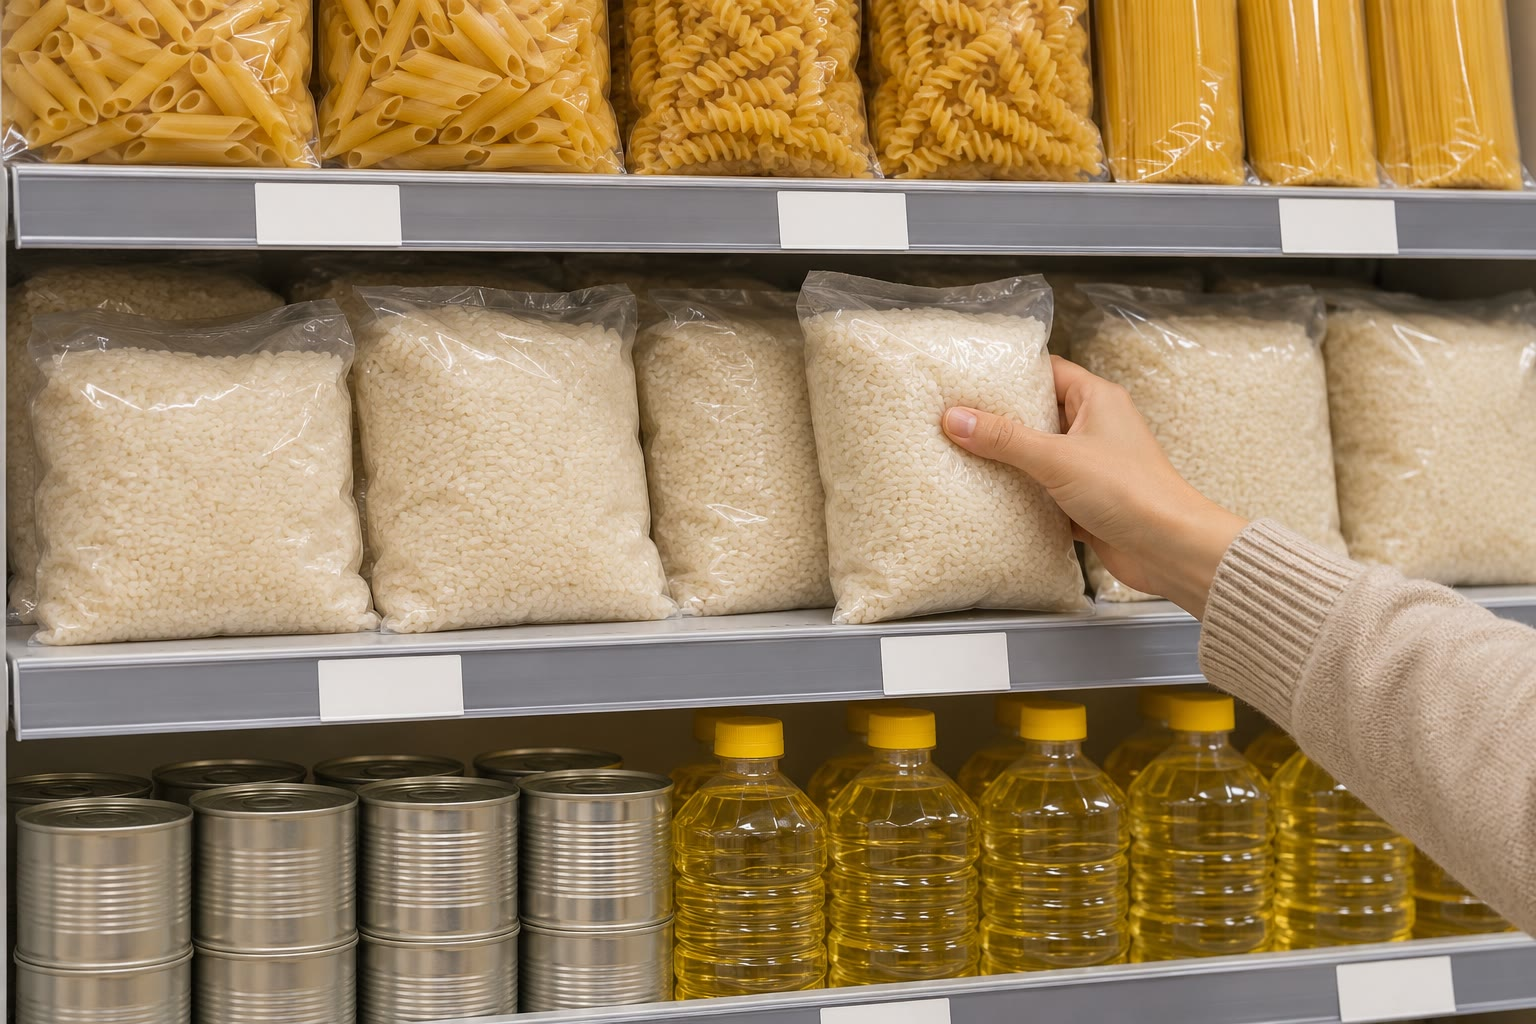
\includegraphics[width=0.48\linewidth]{images/book1/ai/g8-inflation-shop-shelf.jpg}

{\small A supermarket shelf. A \omterm{def:g7:money:price}{price} collector records the \omterm{def:g7:money:price}{price} of the same bag of rice, in the
same shop, every month.}
\end{omfigure}

\section{The inflation rate}

\begin{definition}[Inflation rate]\label{def:g8:inflation-and-price-indices:inflation-rate}
The \emph{inflation rate}\index{inflation rate} over a period is the \omterm{def:g6:reading-economic-charts:rate-of-change}{rate of change} of a \omterm{def:g8:inflation-and-price-indices:price-index}{price
index} over that period, in percent:
\[
\text{inflation rate} = \frac{\text{index at the end} - \text{index at the start}}{\text{index
at the start}} \times 100.
\]
\end{definition}

% figdata: facts (cpi_2024 140.0, cpi_2025 143.5)
Brenland's \omterm{def:g8:inflation-and-price-indices:cpi}{consumer price index} was $140.0$ in 2024 and $143.5$ in 2025 (2015 = 100). Its
\omterm{def:g8:inflation-and-price-indices:inflation-rate}{inflation rate} in 2025 was $(143.5 - 140.0) \div 140.0 = 0.025$, that is $2.5\,\%$. Note that the
index rose by $3.5$ points: points and percent are not the same thing.

\begin{definition}[Deflation]\label{def:g8:inflation-and-price-indices:deflation}
\emph{Deflation}\index{deflation} is a fall in the general level of \omterm{def:g7:money:price}{prices}: a negative
\omterm{def:g8:inflation-and-price-indices:inflation-rate}{inflation rate}.
\end{definition}

Why \omterm{def:g7:money:price}{prices} rise for years, and what the amount of \omterm{def:g7:money:money}{money} has to do with it, is studied in the
volume for grades 10 to 12.

\section{Nominal and real}

\begin{definition}[Nominal value]\label{def:g8:inflation-and-price-indices:nominal}
A \emph{nominal value}\index{nominal value} is an amount of \omterm{def:g7:money:money}{money} measured in the \omterm{def:g7:money:price}{prices} of its
own year.
\end{definition}

\begin{definition}[Real value]\label{def:g8:inflation-and-price-indices:real}
A \emph{real value}\index{real value} is an amount of \omterm{def:g7:money:money}{money} measured in the \omterm{def:g7:money:price}{prices} of a fixed
\omterm{def:g8:inflation-and-price-indices:base-year}{base year}: the \omterm{def:g8:inflation-and-price-indices:nominal}{nominal value} divided by the \omterm{def:g8:inflation-and-price-indices:price-index}{price index}, times 100.
\end{definition}

\begin{definition}[Real wage]\label{def:g8:inflation-and-price-indices:real-wage}
A \emph{real wage}\index{real wage} is a \omterm{def:g7:households:wage}{wage} divided by a \omterm{def:g8:inflation-and-price-indices:cpi}{consumer price index}, times 100: it
measures what the \omterm{def:g7:households:wage}{wage} can buy.
\end{definition}

\begin{example}
A worker in Brenmoor earned $2\,400$ dalens a month in 2015 and $3\,000$ dalens in 2025. The
nominal \omterm{def:g7:households:wage}{wage} rose by $25\,\%$. In 2015 dalens, the 2025 \omterm{def:g7:households:wage}{wage} is worth $3\,000 \div 143.5 \times 100
\approx 2\,091$ dalens: the \omterm{def:g8:inflation-and-price-indices:real-wage}{real wage} fell by $(2\,400 - 2\,091) \div 2\,400 \approx 12.9\,\%$. The
worker is paid more dalens but can buy less.
\end{example}

\begin{definition}[Real GDP]\label{def:g8:inflation-and-price-indices:real-gdp}
\emph{Real GDP}\index{real GDP} is GDP measured in the \omterm{def:g7:money:price}{prices} of a \omterm{def:g8:inflation-and-price-indices:base-year}{base year}, so that its changes
show changes in quantities produced, not in \omterm{def:g7:money:price}{prices}.
\end{definition}

\section{Very high inflation, and falling prices}

\begin{definition}[Hyperinflation]\label{def:g8:inflation-and-price-indices:hyperinflation}
\emph{Hyperinflation}\index{hyperinflation} is inflation so fast that \omterm{def:g7:money:price}{prices} rise by more than
half within a single month.
\end{definition}

\begin{omchart}{Germany's consumer price level, 1914 to 1923 (1914 = 1), on a times-ten scale:
each grid line up multiplies prices by a hundred.}{Jord\`a--Schularick--Taylor Macrohistory Database,
\omterm{def:g8:inflation-and-price-indices:cpi}{consumer price index}, Germany (yearly averages)}
\begin{tikzpicture}
\begin{semilogyaxis}[omtimesten, xmin=1914, xmax=1923, ymin=0.5, ymax=1e12, ytickten={0,2,...,12},
  xtick={1914,...,1923}, xlabel={Year}, ylabel={Price level (1914 = 1)},
  yticklabel={$10^{\pgfmathprintnumber[fixed]{\tick}}$}]
\addplot+[mark=*, mark size=1.5pt] table[x=year, y=level] {figdata/grade-8/03-inflation-and-price-indices/out/germany.csv};
\end{semilogyaxis}
\end{tikzpicture}
\end{omchart}

% figdata: facts (deu_1919 4.0, deu_1922 146, deu_1923 1.55e11)
% ledger: g8:rentenmark-issue, g8:rentenmark-rate, g8:rentenmark-dollar
After the war of 1914--1918, \omterm{def:g7:money:price}{prices} in Germany were four times their 1914 level in 1919, and $146$
times in 1922. In 1923, the year's average was about $1.55 \times 10^{11}$ times the 1914 level:
155 thousand million. On 15 November
1923, a new bank began to issue a new currency, the Rentenmark, worth one trillion ($10^{12}$) old
marks; it was soon held at $4.2$ Rentenmarks to the dollar, and the \omterm{def:g8:inflation-and-price-indices:hyperinflation}{hyperinflation} ended.

\begin{omfigure}
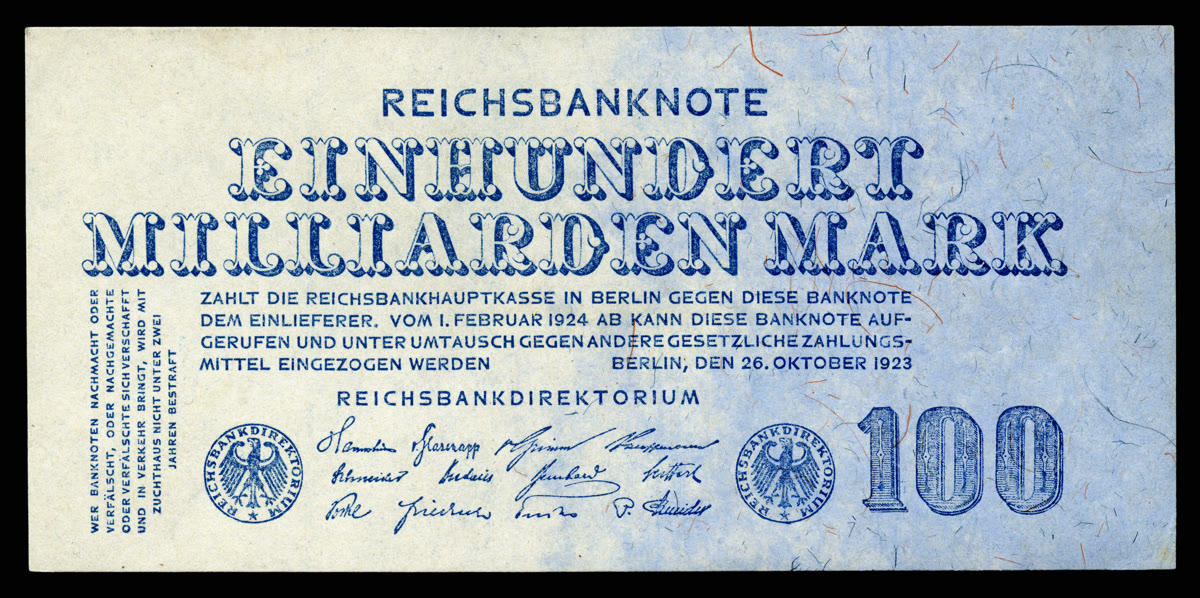
\includegraphics[width=0.58\linewidth]{images/book1/photos/g8-inflation-banknote-1923.jpg}

{\small A German banknote for one hundred thousand million (``hundred milliard'') marks, dated 26
October 1923.}
\end{omfigure}

Falling \omterm{def:g7:money:price}{prices} are rarer. In the United States, \omterm{def:g7:money:price}{prices} fell in 13 of the hundred years of the
opening chart, most of them in the early 1920s and early 1930s. In Japan, \omterm{def:g7:money:price}{prices} fell slightly in
many years after 1995.

\section{Exercises}

\begin{exercise}[$\star$]\label{exo:g8:inflation-and-price-indices:1}
Use the opening chart. About how high was inflation in the United States in 1980?
\end{exercise}

\begin{exercise}[$\star$]\label{exo:g8:inflation-and-price-indices:2}
A \omterm{def:g8:inflation-and-price-indices:basket}{basket} holds 2 kg of rice and 3 litres of oil. In 2020, rice cost $1.50$ dalens a kilogram and
oil $4.00$ dalens a litre; in 2025, $1.80$ and $5.00$. Compute the cost of the \omterm{def:g8:inflation-and-price-indices:basket}{basket} in each
year.
\end{exercise}

\begin{exercise}[$\star$]\label{exo:g8:inflation-and-price-indices:3}
Use exercise 2. Compute the \omterm{def:g8:inflation-and-price-indices:price-index}{price index} for 2025, with 2020 as the \omterm{def:g8:inflation-and-price-indices:base-year}{base year}.
\end{exercise}

\begin{exercise}[$\star$]\label{exo:g8:inflation-and-price-indices:4}
A \omterm{def:g8:inflation-and-price-indices:price-index}{price index} is $118.0$ one year and $123.9$ the next. Compute the \omterm{def:g8:inflation-and-price-indices:inflation-rate}{inflation rate}.
\end{exercise}

\begin{exercise}[$\star\star$]\label{exo:g8:inflation-and-price-indices:5}
Brenland's \omterm{def:g8:inflation-and-price-indices:basket}{basket} costs $10\,850$ dalens at 2015 \omterm{def:g7:money:price}{prices} and $15\,187$ dalens at 2024 \omterm{def:g7:money:price}{prices}.
Compute Brenland's \omterm{def:g8:inflation-and-price-indices:cpi}{consumer price index} for 2024 (2015 = 100), to one decimal.
\end{exercise}

\begin{exercise}[$\star\star$]\label{exo:g8:inflation-and-price-indices:6}
A nurse earns $3\,400$ dalens a month in 2025, when Brenland's index is $143.5$ (2015 = 100). What
is the \omterm{def:g7:households:wage}{wage} in 2015 dalens?
\end{exercise}

\begin{exercise}[$\star\star$]\label{exo:g8:inflation-and-price-indices:7}
Use the opening chart. In which periods of the 1920s and 1930s did \omterm{def:g7:money:price}{prices} fall in the United
States?
\end{exercise}

\begin{exercise}[$\star\star$]\label{exo:g8:inflation-and-price-indices:8}
In a \omterm{def:g8:inflation-and-price-indices:hyperinflation}{hyperinflation}, \omterm{def:g7:money:price}{prices} double every month for a year. By how many times are \omterm{def:g7:money:price}{prices} higher at
the end of the year? Write the answer as a power of 2, then as a number.
\end{exercise}

\begin{exercise}[$\star\star$]\label{exo:g8:inflation-and-price-indices:9}
The \omterm{def:g8:inflation-and-price-indices:cpi}{consumer price index} keeps the same \omterm{def:g8:inflation-and-price-indices:basket}{basket} for several years. Give two reasons why it might
overstate how much the cost of living of a \omterm{def:g7:households:household}{household} has risen.
\end{exercise}

\begin{exercise}[$\star\star\star$]\label{exo:g8:inflation-and-price-indices:10}
Brenland's GDP was $183\,201$ million dalens in 2005 and $393\,264$ million in 2025. Its GDP \omterm{def:g8:inflation-and-price-indices:price-index}{price
index} was $84.6$ in 2005 and $134.5$ in 2025 (2015 = 100). (a) By how many times did nominal GDP
grow? (b) Compute \omterm{def:g8:inflation-and-price-indices:real-gdp}{real GDP} in 2015 dalens in both years. (c) By what percentage did \omterm{def:g8:inflation-and-price-indices:real-gdp}{real GDP} grow?
\end{exercise}

\begin{exercise}[$\star\star\star$]\label{exo:g8:inflation-and-price-indices:11}
Use the text on Germany. (a) By about how many powers of ten were \omterm{def:g7:money:price}{prices} higher in 1923 than in
1914? (b) How many times higher were they in 1923 than in 1922, as a power of ten?
\end{exercise}

\begin{exercise}[$\star\star\star$]\label{exo:g8:inflation-and-price-indices:12}
The \omterm{def:g8:inflation-and-price-indices:cpi}{consumer price index} rose by $2.5\,\%$ in a year. Explain why the \omterm{def:g7:money:price}{prices} paid by one particular
family may have risen by much more, or much less.
\end{exercise}

\section{Problem: The Brenmoor Basket}

\begin{problem}[{Weekend problem --- pricing Brenland's 2015 basket, the index and inflation, and
a wage in real terms}]
\label{pb:g8:inflation-and-price-indices:1}
% figdata: basket (qty 300 12 100 20 3000; p2015 2 700 3 40 0.25; p2024 2.68 973.33 3.82 48.55 0.45;
% p2025 2.71 1000.14 3.91 49 0.46)
Brenland's \omterm{def:g8:inflation-and-price-indices:cpi}{consumer price index} \omterm{def:g7:money:price}{prices} this \omterm{def:g8:inflation-and-price-indices:basket}{basket}, bought by a \omterm{def:g7:households:household}{household} in a year (invented
data). \omterm{def:g7:money:price}{Prices} are in dalens per unit. It holds five goods only, not a full \omterm{def:g8:inflation-and-price-indices:basket}{basket}: food other than
bread, and most other goods and services, are left out, so rent weighs much more here than it
would in a real index: in the United States, housing takes $30$ to $43\,\%$ of \omterm{def:g7:households:household}{households}'
spending (\cref{ch:g7:households}).
\begin{center}
\begin{tabular}{lrrrr}
\toprule
Good & Quantity & \omterm{def:g7:money:price}{Price} 2015 & \omterm{def:g7:money:price}{Price} 2024 & \omterm{def:g7:money:price}{Price} 2025 \\
\midrule
Bread (loaves) & 300 & $2.00$ & $2.68$ & $2.71$ \\
Rent (months) & 12 & $700.00$ & $973.33$ & $1\,000.14$ \\
Transport (tickets) & 100 & $3.00$ & $3.82$ & $3.91$ \\
Clothing (items) & 20 & $40.00$ & $48.55$ & $49.00$ \\
Energy (kWh) & $3\,000$ & $0.25$ & $0.45$ & $0.46$ \\
\bottomrule
\end{tabular}
\end{center}

\medskip
\noindent\textbf{Part I --- The basket in 2015.}
\begin{enumerate}
  \item Compute the cost of each good in the \omterm{def:g8:inflation-and-price-indices:basket}{basket} at 2015 \omterm{def:g7:money:price}{prices}.
  \item Compute the cost of the whole \omterm{def:g8:inflation-and-price-indices:basket}{basket} in 2015.
  \item What share of the \omterm{def:g8:inflation-and-price-indices:basket}{basket}'s cost is rent, in percent, to one decimal?
  \item Compute the weight of each of the other four goods, in percent, to one decimal.
\end{enumerate}

\medskip
\noindent\textbf{Part II --- The index.}
\begin{enumerate}[resume]
  \item Compute the cost of the \omterm{def:g8:inflation-and-price-indices:basket}{basket} at 2025 \omterm{def:g7:money:price}{prices}.
  \item Compute the \omterm{def:g8:inflation-and-price-indices:cpi}{consumer price index} for 2025 (2015 = 100), to one decimal.
  \item Compute the rise in the \omterm{def:g7:money:price}{price} of each good from 2015 to 2025, in percent, to one decimal.
  \item Explain why the index rose by almost as much as rent, although energy rose much more.
  \item The index was $140.0$ in 2024. Compute the \omterm{def:g8:inflation-and-price-indices:inflation-rate}{inflation rate} in 2025.
\end{enumerate}

\medskip
\noindent\textbf{Part III --- A wage in real terms.} A bus driver earned $2\,400$ dalens a month in
2015 and $3\,600$ dalens in 2025.
\begin{enumerate}[resume]
  \item By what percentage did the nominal \omterm{def:g7:households:wage}{wage} rise?
  \item Compute the 2025 \omterm{def:g7:households:wage}{wage} in 2015 dalens, to the nearest dalen.
  \item The driver owns a home and pays no rent. \omterm{def:g7:money:price}{Price} the rest of the \omterm{def:g8:inflation-and-price-indices:basket}{basket} in 2015 and 2025: by
        what percentage did its cost rise?
  \item Using the index, by what percentage did the driver's \omterm{def:g8:inflation-and-price-indices:real-wage}{real wage} change from 2015 to 2025?
\end{enumerate}
\end{problem}
